%%%%%%%%%%%%%%%%%%%%%%%%%%%%%%%%%%%%%%%%%%%%%%%%%%%%%%
\chapter{General introduction}
\label{general_introduction}
\graphicspath{{chapter_01/figures}{chapter_01/tables}}
%%%%%%%%%%%%%%%%%%%%%%%%%%%%%%%%%%%%%%%%%%%%%%%%%%%%%%



\chapterindent Flash \marginpara{The socio-economic impacts of flash floods} floods represent the deadliest and most devastating form of natural hazard, causing over 5,000 fatalities annually and accounting for approximately 85\% of global flood incidents \citep{Dordevic_2020}. The impact of flash floods extends across urban and rural landscapes, profoundly affecting lives, livelihoods, and critical infrastructure worldwide \citep{Liu_2024a}. The socio-economic \citep{Ebi_2021} and environmental \citep{Zhang_2024a} impacts of flash floods can be severe and transcend the traditional divide between developed and developing countries. In October 2024, flash floods in Valencia, Spain, claimed more than 200 lives and caused extensive damage in 87 municipalities \citep{Grau-Bove_2024}, while between March and September 2024, sustained periods of intense rainfall and subsequent flash flooding in Pakistan and Afghanistan resulted in 1084 deaths, 2600 injuries, and extensive damage to houses \citep{Wikipedia_2025}. In low- and middle-income countries in Africa, Latin America, and Asia, flash floods can also exacerbate existing socio-economic and environmental vulnerabilities to the extent of displacing entire populations \citep{Stephens_2024} or undermining food security and food safety \citep{Agabiirwe_2022, Duchenne-Moutien_2021}. Impacts from flash floods are more severe primarily due to rapid, unregulated urbanisation in flood-prone areas, limited infrastructure for flood management, insufficient early warning systems, and economic constraints on implementing preventive measures \citep{Douglas_2017, Pinos_2022, Wang_2021b}. Regions affected by flash floods can also be vulnerable to waterborne diseases with outbreaks of cholera, typhoid, and other infectious diseases due to flood waters contaminating drinking water sources or overwhelming sanitation systems \citep{Lee_2020}. Populations affected by extremely severe flash floods may also experience serious psychological impacts, including anxiety, depression, and post-traumatic stress disorder \citep{Iqbal_2023}. 

As \marginpara{On the urgent need for accurate, timely, and scalable flash flood forecasts} climate change increases the frequency and intensity of extreme rainfall \citep{WMO_2025, IPCC_2023}, also in historically low-risk regions \citep{Fowler_2021c}, a comprehensive re-evaluation of risk management, adaptation, and mitigation frameworks is needed to protect vulnerable communities. Recognising their severe and growing impacts, WMO targets flash floods as one of its top priority natural hazards \citep{WMO_2025}. The UN's 'Early Warnings for All' initiative, launched in 2022 and aiming to protect every person on Earth with early warning systems by 2027, also places flash floods at the forefront of its agenda \citep{UN_2022}. Forecasts with global coverage that are accurate and timely (e.g. several days in advance) are crucial to the success of such an initiative as they could enable targeted protective decisions worldwide \citep{Merz_2020}, including in regions where longer lead times are crucial for mobilising resources and executing emergency plans \citep{Bazo_2019}. 

Despite \marginpara{Current challenges in flash flood forecasting: scaling predictions for large domains and extending lead times} general advances in flash flood prediction (for example, the development of high-resolution physical and data-driven NWP and hydrological models), significant technical and methodological obstacles persist for the development of medium-range flash flood forecasts (i.e. up to 10 days ahead), over a continuous global domain \citep{Zanchetta_2020}. Such obstacles include inherent uncertainty in extreme localised rainfall forecasts beyond a few hours, computational demands running high-resolution models over large domains, and limited availability of real-time hydro-meteorological observations. These limitations affect the ability to predict flash floods with sufficient lead time and over a continuous large-scale (e.g., global domain), leaving many regions unprotected \citep{AlRawas_2024}. The WMO's Flash Flood Guidance System attempts to address the patchy spatial coverage of flash flood forecasting systems \citep{Georgakakos_2022}. This initiative focuses, however, on implementing distinct regional systems around the world, not fully resolving the issue of inconsistent coverage. Furthermore, the system's reliance on high-density observational networks, km-scale NWP model outputs, and high computational costs compromise its scalability in regions with limited resources. Therefore, developing robust medium-range flash flood forecasting capabilities at global scale remains one of the pressing challenges of modern hydrology.

The \marginpara{Opportunities for global medium-range flash flood forecasts: proven effectiveness of index-based systems over large-scale domains, enhanced quality of medium-range global NWP rainfall predictions, and emergence of data-driven approaches for hydrological applications} unprecedented convergence of three key scientific advancements over the last decade has created a unique opportunity to develop medium-range flash flood forecasts with global coverage. Index-based flash flood forecasting systems, focusing on key variables like rainfall and soil moisture, have proven more effective and computationally efficient at national and continental scales than complex physically-based models  \citep{Alfieri_2015a}. However, their reliance on high-resolution, short-range rainfall forecasts from radars or km-scale NWP models still limits their spatial coverage to data-rich regions like Europe and the US, and restricts forecasts lead times to nowcasting time scales (i.e. a few hours), thereby reducing available preparedness and response time \citep{Luong_2021, Maybee_2024}. Over the past decade, global (ensemble) NWP models have significantly improved their ability to forecast extreme rainfall up to the medium-range lead times \citep{Lavers_2021, Haiden_2023}. Despite their coarse spatial resolution (typically >10 km), there is growing interest in testing global NWP forecasts for flash flood applications and extending prediction lead times \citep{Bucherie_2022b}. Moreover, statistical post-processing techniques make these predictions more palatable for flash flood forecasting \citep{Vannitsem_2021}. The recent success of data-driven approaches in predicting riverine floods \citep{Nearing_2024} has increased the interest in extending their application to flash flood forecasting. Notwithstanding the innovative paradigm of \textit{training a model where data is available and applying it globally} \citep{Kratzert_2024}, the paucity of observational data suitable for flash flood modelling continues to hinder the development of data-driven approaches for large-scale flash flood forecasting \citep{Alzubaidi_2023}. When run using global medium-range NWP model outputs, simpler machine learning models (e.g., decision-tree-based algorithms or feed-forward neural networks), optimised for sparse and imbalanced datasets and informed by physical insights from index-based models, may enable the development of the first prototype medium-range flash flood prediction system with true global coverage.


%%%%%%%%%%%%%%%%%%%%%%%%%%%%%%%%%%%%%%%%%%%
\section{Research Objectives and Questions}
\label{general_introduction_research_objectives_questions}

While \marginpara{Develop a flash-flood-focused verification framework to assess whether global NWP rainfall forecasts can identify areas at risk of flash flood} new global NWP rainfall forecasts are regularly developed, their effectiveness in identifying areas at risk of flash floods remains largely untested. Most verification efforts focus on comparing predicted rainfall against rainfall observations, operating under the implicit assumption that improved rainfall forecasts will translate into better flash flood prediction capabilities \citep{Gascón_2024}. The primary objective of this thesis is to depart from the traditional rainfall-to-rainfall verification approach and adopt, instead, a flash-flood-focused framework that directly compares ecPoint rainfall forecasts with flash flood observations (e.g. discharge or impact reports) to determine whether state-of-the-art global NWP rainfall forecasts can serve as a basis for global flash flood prediction up to medium-range lead times. Key challenges include designing metrics to account for the differences between continuous rainfall predictions and binary flash flood occurrences, addressing spatial and temporal uncertainties in flash flood reporting, and establishing meaningful performance measures applicable across diverse rainfall climatologies. This thesis will employ the \textit{global ecPoint rainfall forecasts}, which represent the current state-of-the-art in post-processed global NWP rainfall predictions for localised extreme events, having demonstrated significant skill improvements over raw global NWP predictions through their post-processing approach \citep{Hewson_2021}. It is also worth highlighting that, due to the severe underrepresentation of flash flood events in global (hydrological or impact) databases, this research will develop the verification framework as a \textit{regional prototype} over the CONtiguous US (CONUS), where a high-density, detailed \textit{flash flood impact database} is available, i.e. NOAA's Storm Event Database. The outcomes of this flash-flood-focused verification framework will provide insights into the effectiveness of state-of-the-art post-processed NWP rainfall forecasts in identifying areas at risk of flash floods. It will also serve as a performance baseline for the verification analysis in subsequent chapters, where data-driven predictions of areas at risk of flash floods that incorporate hydro-meteorological variables will be developed. \textbf{Research Question n.1 (RQ1): Can post-processed global NWP rainfall forecasts successfully identify areas at risk of flash floods up to medium-range lead times?}

Despite \marginpara{Assess the feasibility of developing data-driven models for global flash flood prediction using hydro-meteorological reanalysis data} the recent surge in data-driven applications for riverine flood prediction in large-sample hydrology \citep{Nearing_2024}, data-driven flash flood prediction remains confined at catchment level \citep{Ding_2025, Zhao_2025, Song_2020, Saleh_2024} or national scale \citep{Zhao_2022}, with lead times limited to 24 hours. The development of medium-range, global data-driven flash flood prediction systems has been hindered by the \textit{severe class imbalance} inherent in flash flood datasets, where events typically represent less than 1\% of observational records \citep{Kratzert_2023, Färber_2024, Panwar_2020, Jonkman_2024}. The second research objective of this thesis aims to address these limitations by assessing the feasibility of developing data-driven models for predicting areas at risk of flash floods. The methodological framework must overcome three fundamental challenges. First, model selection (whether tree-based ensembles or neural networks) must account for extreme class imbalance, high-dimensional feature spaces, and operational computational constraints. The architectural design must also prioritise both predictive accuracy and operational feasibility. Whilst deep learning approaches have revolutionised many domains of environmental prediction \citep{Lang_2024, Nearing_2024}, evidence suggests that parsimonious architectures, such as regularised ensemble methods and shallow neural networks, may outperform deep learning architectures for severely imbalanced datasets \citep{Kumar_2021, Xu_2022, Luo_2025a}.  Second, feature engineering must identify the most informative hydro-meteorological predictors whilst maintaining model interpretability and computational efficiency. Third, uncertainty quantification through ensemble modelling becomes essential for providing reliable risk estimates \citep{Saleh_2024}. The proposed methodology will utilise ERA5 reanalysis data (i.e. short-range forecasts, up to day 0) for hydro-meteorological features and flash flood impact reports from NOAA's Storm Event Database, thereby implementing a regional prototype over CONUS. The development process will encompass a systematic literature review for predictor selection, architectural design optimisation, and validation against the rainfall-based predictions established in the first research objective. Whilst initially regional in scope, sensitivity analyses will explore the requirements for global extension of the methodology. \textbf{Research Question n.2 (RQ2): Is it feasible to develop data-driven predictions of areas at risk of flash flood at regional/global scale using reanalysis hydro-meteorological data and impact flash flood reports?}

Whilst \marginpara{Evaluate the predictability of medium-range data-driven predictions of areas at risk of flash flood using medium-range global NWP hydro-meteorological forecasts} the application of short-range (i.e., reanalysis) hydro-meteorological data may demonstrate the feasibility of identifying areas at risk of flash floods at very short lead times (up to day 0), the extension of data-driven methodologies to medium-range timescales remains unexplored. Recent advances in data-driven forecasting of rare atmospheric phenomena, such as lightning, that face similar challenges to flash floods regarding extreme class imbalance and spatio-temporal variability, demonstrate sustained predictive skill up to 48 hours \citep{Cavaiola_2024}. These findings suggest that data-driven approaches may extend the predictability horizon for flash floods beyond current operational capabilities (i.e. 24 hours) to provide the needed temporal window for implementing effective mitigation strategies and coordinating emergency response protocols. The third research objective addresses this gap by systematically evaluating the predictability of data-driven flash flood forecasts at medium-range timescales, using global NWP hydro-meteorological data from ERA5's long-range forecasts (up to day 5)\footnote{The terminology "short-range" and "long-range" forecasts follows ECMWF's official nomenclature for ERA5 products. Within this framework, "short-range" refers to the ERA5's 0-18 hour forecasts used to create the reanalysis data, whilst "long-range" denotes predictions extending to day 10. This convention differs from the broader meteorological usage of the "long-range" term, which typically implies seasonal timescales. Chapter \ref{datasets} will provide comprehensive descriptions of both short- and long-range ERA5 forecast.}. Building upon the modelling framework established in the second research objective, this investigation will evaluate the medium-range data-driven predictions of areas at risk of flash floods following two complementary approaches. First, an objective verification framework will be implemented over CONUS, enabling a quantitative assessment of forecast skill degradation with increasing lead time and direct comparison with the performance of the short-range data-driven predictions as well as the medium-range rainfall-based predictions of areas at risk of flash floods. This analysis will establish the temporal limits of predictability and quantify the growth of uncertainty across the forecast horizon. Second, a subjective verification approach employing targeted case studies will be conducted across diverse global hydro-climatic regions, providing qualitative insights into model performance under varying environmental conditions and flash flood generation mechanisms. Together, these analyses will determine the operational utility of medium-range data-driven flash flood forecasts for supporting risk-informed decision-making in emergency management contexts. \textbf{Research Question n.3 (RQ3): What is the predictability of data-driven predictions of areas at risk of flash floods at medium-range lead times, at regional/global scale?}


%%%%%%%%%%%%%%%%%%%%%%%%%%%%%%%%%%%%%%%%%%%%%%%%%%%%%%%%%%%%%%%%%%%%%%%%%%%
\section{Contributions to knowledge and practice in flash flood prediction}
\label{general_introduction_contribution_to_knowledge}

This thesis contributes to the scientific understanding of predictive capabilities and methodological constraints in developing medium-range predictions of areas at risk of flash floods over a continuous global domain. The research in this thesis progresses through three interconnected research questions (RQ), each building upon the findings and methodological insights of its predecessor.

By addressing RQ1\marginpara{Contribution to knowledge no. 1: creation of a flash-flood-focused verification framework and a benchmark verification dataset for data-driven predictions based on hydro-meteorological parameters}, this thesis introduces a \textit{flash-flood-focused verification framework}, a methodology that directly compares global NWP rainfall predictions with observed flash flood occurrences. Departing from conventional rainfall-to-rainfall verification paradigms, this contribution addresses a methodological gap in the literature given by the implicit assumption that improved rainfall forecasts necessarily enhance flash flood predictions. By implementing this direct comparison between global NWP rainfall predictions and observed flash flood occurrences, we provide empirical evidence of whether advances in numerical weather prediction modelling translate to enhanced flash flood predictability up to medium-range timescales. The investigation employs the CONUS as the primary experimental domain, leveraging the exceptional spatio-temporal resolution and completeness of NOAA's Storm Event Database for objective verification. Moreover, the outcomes of this phase provide a performance benchmark for the short- and medium-range data-driven flash flood predictions that will be developed at the later stages of this research. 

By addressing RQ2\marginpara{Contribution to knowledge no. 2: feasibility of data-driven flash flood prediction models}, this thesis examines the feasibility of developing data-driven predictions of areas at risk of flash floods using hydro-meteorological data from ERA5's short-range forecasts (day 0) and flash flood impact observations. In this stage, we will explore different data-driven algorithms, feature selection, and training methodologies. The outcomes of this stage will also provide critical insights on the benefits and limitations of these advanced data-driven systems, incorporating multiple hydro-meteorological variables, through the comparative assessment of the rainfall-based predictions introduced in the previous phase. As mentioned above, the investigation employs the CONUS as the primary experimental domain. A sensitivity analysis was, however, carried out to investigate which data approach would be more appropriate to extend regional training to create predictions over a continuous global domain. A subjective analysis, based on flash floods case studies over different continents complement the regional objective verification analysis, illustrating the benefits and limitations of the global extension of the regional training. In conclusion, this research would offer a pathway for scalable flash flood early warning systems with true global coverage, particularly valuable where traditional forecasting methods face data or computational limitations. Moreover, the outcomes of this research would align with the UN's "Early Warnings for All" initiative by potentially extending life-saving warnings to historically underserved communities.

By addressing RQ3\marginpara{Contribution to knowledge no. 3: predictability of data-driven flash flood forecasts at medium-range lead times}, this thesis evaluates the medium-range, data-driven predictions of areas at risk of flash floods using hydro-meteorological data from ERA5's long-range forecasts and flash flood impact data. Thus, this research explores the practical opportunities and challenges of extending flash flood predictions beyond traditional short lead times (up to t+24). In this stage, these medium-range forecasts are benchmarked against the data-driven short-range forecasts developed to address RQ2 and the short- and medium-range rainfall-based forecasts assessed to address RQ1. In this way, the added value of complex machine learning frameworks despite their increased computational and data requirements and their potential limitations arising from uncertainty propagation in hydro-meteorological variables at extended lead times is assessed.


%%%%%%%%%%%%%%%%%%%%%%%%%%%%%%%%%%%%%%%%%%%
\section{Thesis Structure and Organisation}
This thesis is divided into the following nine chapters:

\begin{figure}[htbp]
\centering
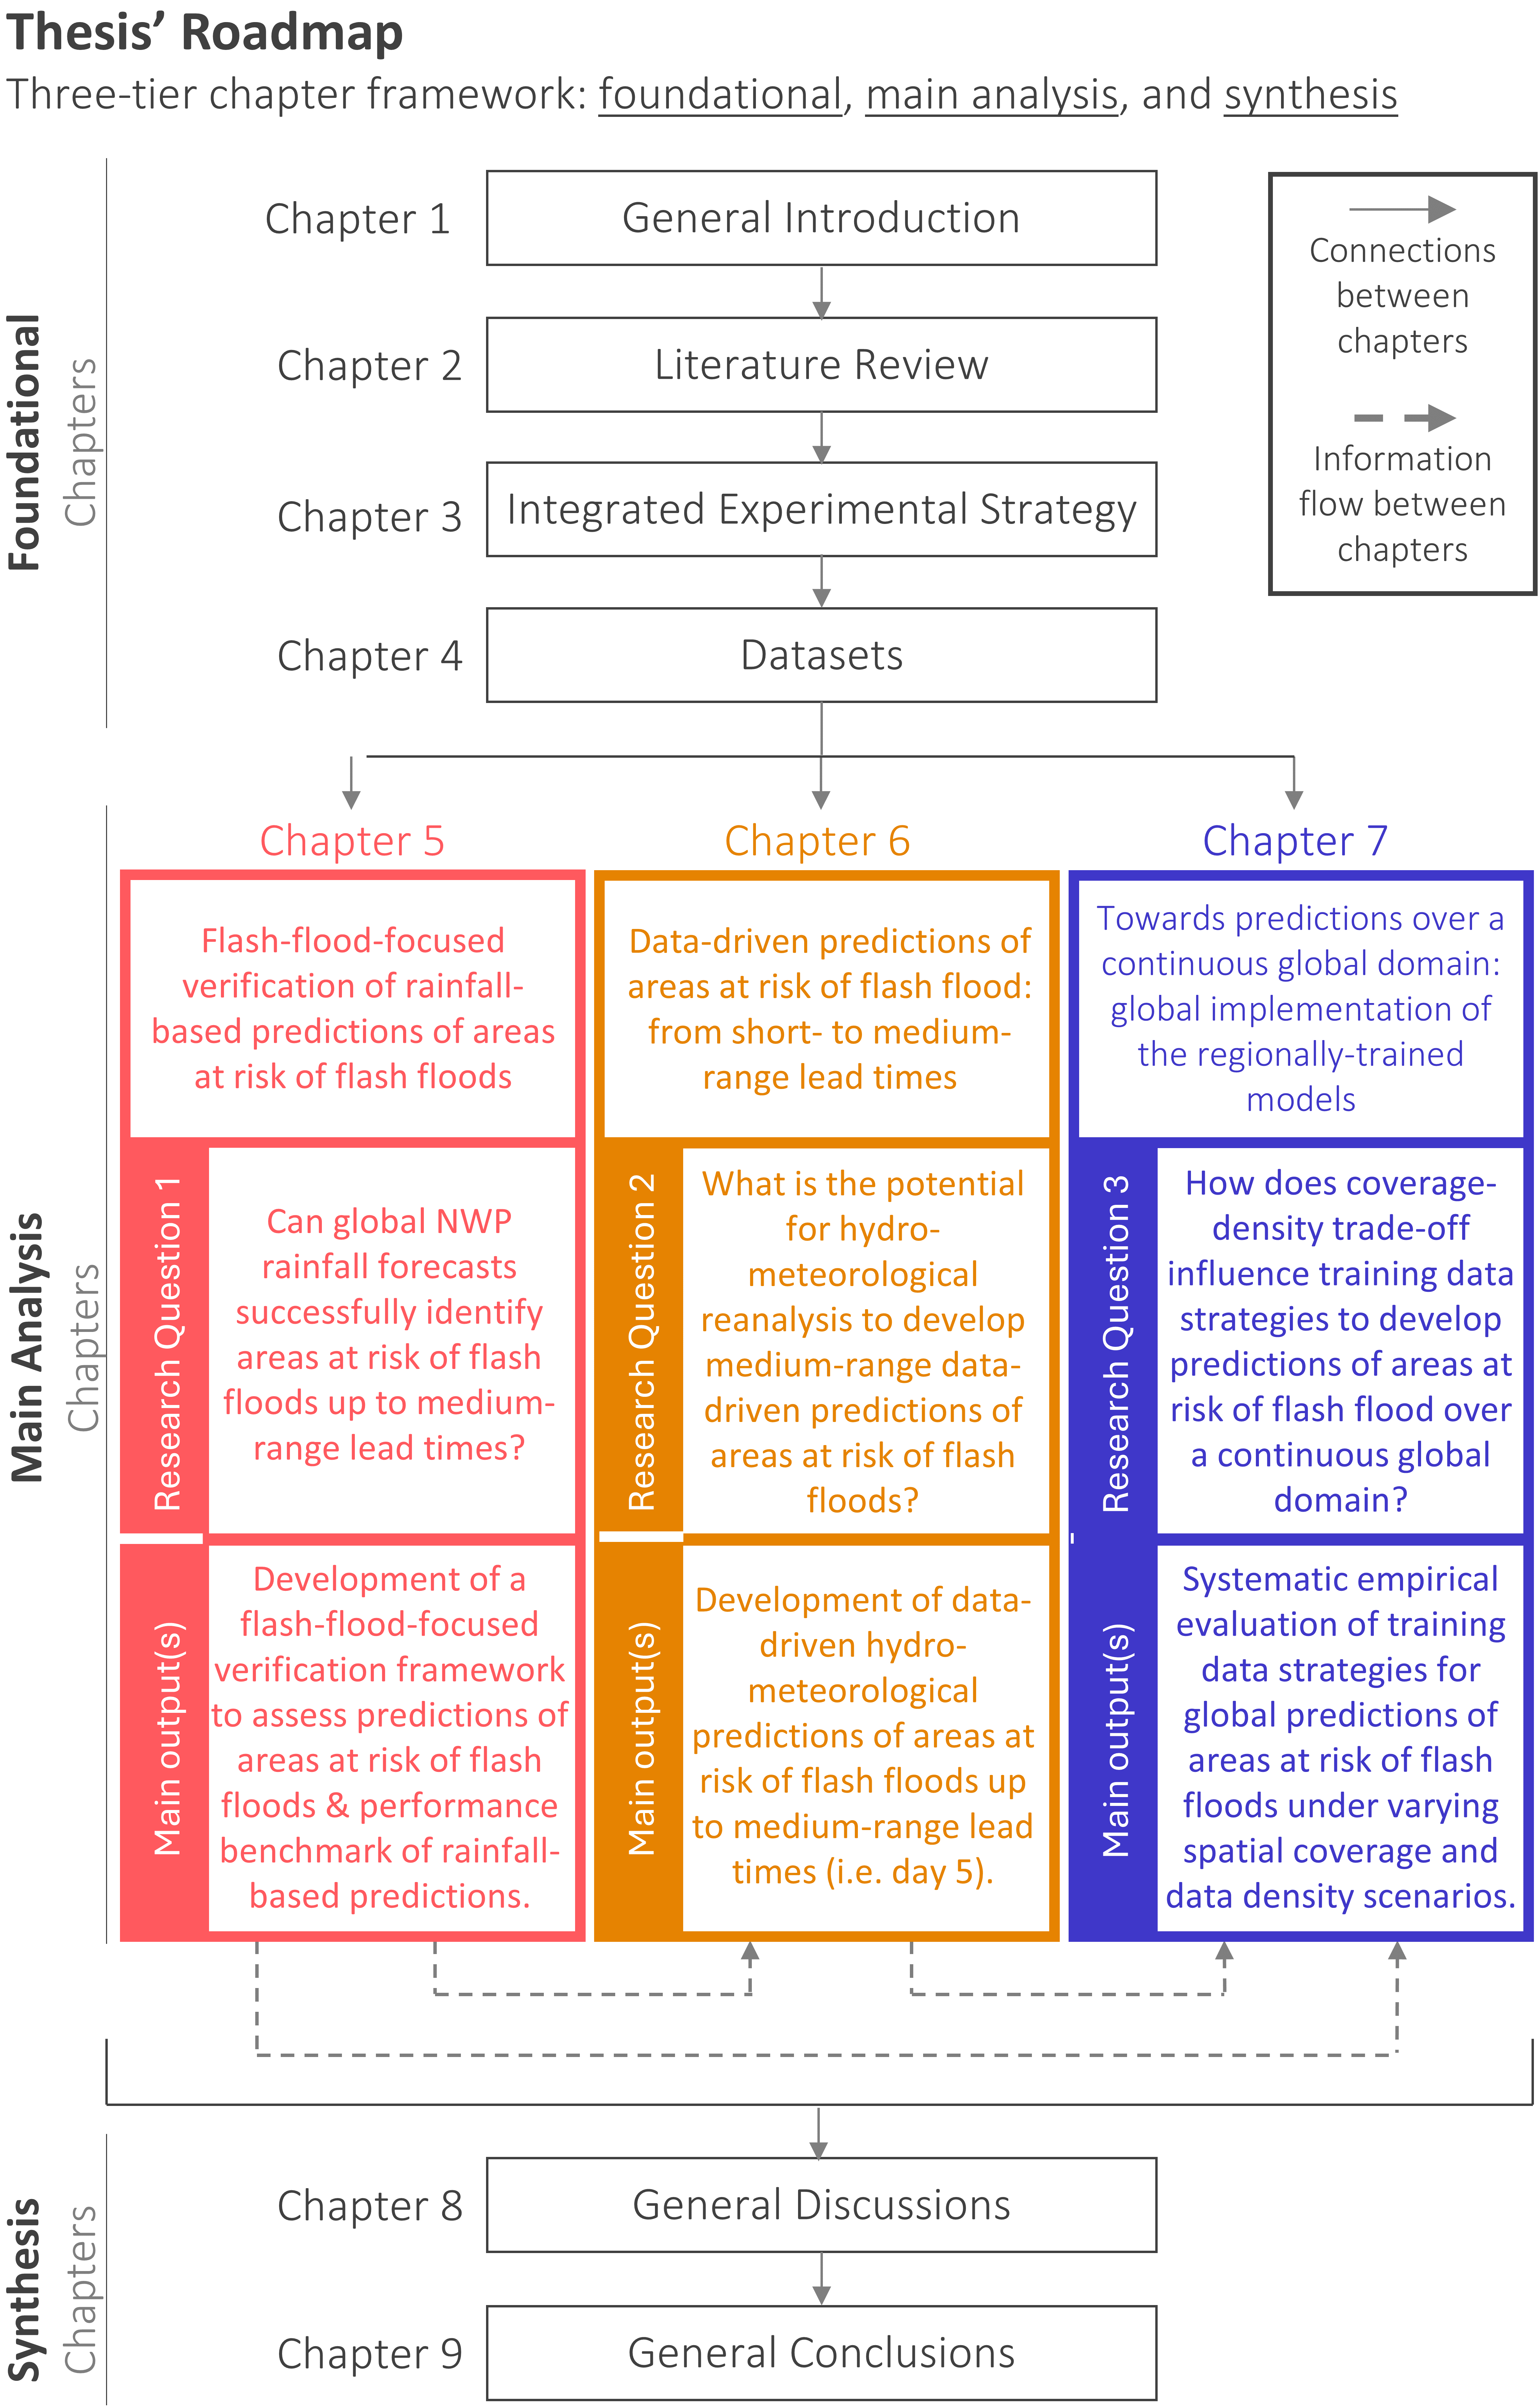
\includegraphics[width=\textwidth]{thesis_roadmap.png}
\caption{\textbf{Overview of the thesis structure.} It illustrates the progression from the \textit{Foundational Chapters} (General Introduction - Chapter 1; Literature Review - Chapter 2; Experimental Design - Chapter 3; Datasets - Chapter 4), followed by the \textit{Main Analysis Chapters} (Flash-Flood-Focused Rainfall Verification - Chapter 5, indicated in pink; Feasibility of Data-Driven Flash-Flood Prediction Models - Chapter 6, indicated in orange; Predictability of Data-Driven Flash-Flood Forecasts - Chapter 7, indicated in blue), and concluding with the \textit{Synthesis Chapters} (General Discussions - Chapter 9; General Conclusions - Chapter 10).}
\label{fig:thesis_structure}
\end{figure}

\textbf{Chapter 1}\marginpara{Foundational Chapter - General Introduction} established the foundation for this research by addressing the critical need for improved flash flood early warning systems worldwide. The chapter presented the three interconnected research questions addressed in this thesis, i.e., the development of a flash-flood-focused verification framework to assess the performance of global NWP rainfall forecasts in the prediction of areas at risk of flash flood, the creation of data-driven flash flood prediction models using reanalysis data, and the analysis of their predictability up to medium-range lead times. It also introduced the contributions to knowledge and practice in flash flood prediction done by this research that will be further discussed in section \ref{general_discussion_contribution_Knowledge}.

\textbf{Chapter 2}\marginpara{Foundational Chapter - Literature Review} presents a synthesis of the scientific literature in flash flood prediction, establishing the theoretical foundations and delineating the methodological gaps addressed by the three research questions presented in section \ref{general_introduction_research_objectives_questions}.

\textbf{Chapter 3}\marginpara{Foundational Chapter - Experimental Design} delineates the experimental design through which the three research questions are systematically addressed, demonstrating their sequential dependencies and synergistic relationships.

\textbf{Chapter 4}\marginpara{Foundational Chapter - Datasets} presents the datasets considered to address the three presented research questions. It presents the short- and long-range ERA5 rainfall forecasts, post-processed with the ecPoint technique. It also presents the short- and long-range ERA5 forecasts for the soil water content, considered to represent soil's moisture conditions prior the flash flood events. It also presents the climatological parameter characterising the terrain vegetation coverage (i.e., leaf area index), and the static fields representing its steepness (i.e., slope of the sub-grid orography and standard deviation of the filtered sub-grid orography). Moreover, the chapter presents the flash flood impact database used throughout this thesis, NOAA's Storm Event Database, discussing their geographical coverage over the CONUS, its temporal resolution, and its inherent reporting limitations. 

\textbf{Chapter 5}\marginpara{Main Analysis Chapter - Flash-Flood-Focused Rainfall Verification}
introduces a robust flash-flood-focused verification methodology to evaluate the performance of global NWP rainfall forecasts in identifying areas at risk of flash floods, contributing to answering RQ1. The methodology directly verifies rainfall forecasts against flash flood impact observations, addressing challenges such as the interpretation of metrics for dissimilar quantities and managing unreported events. Long-term objective verification and case studies validate the framework while revealing the strengths and limitations of global NWP rainfall forecasts for flash flood prediction. 

\textbf{Chapter 6}\marginpara{Main Analysis Chapter - Feasibility of Data-Driven Flash Flood Prediction Models} examines the feasibility of developing data-driven flash flood prediction models using global ERA5 hydro-meteorological short-range forecasts (up to day 0). The research presents innovative data-driven architectures designed to process ERA5 hydro-meteorological data, carefully considering predictor selection, training strategies, and uncertainty assessment methodologies. Utilising NOAA's Storm Event Database over the contiguous US, the models undergo rigorous validation through both objective score-based verification and subjective case-study analysis following the flash-flood-focused verification framework developed in Chapter 5. The chapter further explores the models' transferability to different geographical regions and climate conditions through sensitivity analyses.

\textbf{Chapter 7}\marginpara{Main Analysis Chapter - Predictability of Data-Driven Flash Flood Forecasts} assesses the predictability of data-driven flash flood forecasts up to medium-range lead times, using ERA5 hydro-meteorological long-range forecasts (from day 1 to day 5), and following the flash-flood-focused verification framework developed in Chapter 5. Building on the data-driven flash flood prediction model developed in Chapter 6, this investigation addresses the challenges of utilising forecast data, including prediction uncertainty and reliability across various lead times through objective verification and case studies. 

\textbf{Chapter 8}\marginpara{Synthesis Chapter - General Discussions} synthesises and discusses the research findings in the main analysis chapters, critically evaluating how effectively each research question was addressed. The chapter explores the broader implications for disaster risk reduction and emergency management, exploring how these advancements may enhance global early warning capabilities against the impacts of flash floods. 

\textbf{Chapter 9}\marginpara{Synthesis Chapter - General Conclusions} concludes the thesis by articulating its novel contributions to flash flood prediction knowledge and practice. It provides final assessments for each research question, acknowledging methodological limitations whilst clearly stating the scientific advancements achieved. The chapter concludes by exploring future research directions that might strengthen the use of forecasts from global NWP models and data-driven approaches for predicting flash floods over a continuous global domain up to medium-range lead times. 